%%%%%%%%%%%%%%%%%%%%%%%%%%%%%%%%%%%%%%%%%%%%%%%%%%%%%%%%%%%%%%%%%%%%%%%%

%%% LaTeX Template for AAMAS-2026 (based on sample-sigconf.tex)
%%% Prepared by the AAMAS-2026 Publication Chairs based on the version from AAMAS-2025. 

%%%%%%%%%%%%%%%%%%%%%%%%%%%%%%%%%%%%%%%%%%%%%%%%%%%%%%%%%%%%%%%%%%%%%%%%

%%% Start your document with the \documentclass command.


%%% == IMPORTANT ==
%%% Use the first variant below for the final paper (including author information).
%%% Use the second variant below to anonymize your submission (no author information shown).
%%% For further information on anonymity and double-blind reviewing, 
%%% please consult the call for paper information
%%% https://cyprusconferences.org/aamas2026/submission-instructions/

%%%% For anonymized submission, use this
\documentclass[sigconf,anonymous]{aamas} 

%%%% For camera-ready, use this
%\documentclass[sigconf]{aamas} 


%%% Load required packages here (note that many are included already).

\usepackage{balance} % for balancing columns on the final page

\newcommand{\ykc}[1]{{\color{blue} #1}}

%%%%%%%%%%%%%%%%%%%%%%%%%%%%%%%%%%%%%%%%%%%%%%%%%%%%%%%%%%%%%%%%%%%%%%%%

%%% AAMAS-2026 copyright block (do not change!)

\setcopyright{ifaamas}
\acmConference[AAMAS '26]{Proc.\@ of the 25th International Conference
on Autonomous Agents and Multiagent Systems (AAMAS 2026)}{May 25 -- 29, 2026}
{Paphos, Cyprus}{C.~Amato, L.~Dennis, V.~Mascardi, J.~Thangarajah (eds.)}
\copyrightyear{2026}
\acmYear{2026}
\acmDOI{}
\acmPrice{}
\acmISBN{}


%%%%%%%%%%%%%%%%%%%%%%%%%%%%%%%%%%%%%%%%%%%%%%%%%%%%%%%%%%%%%%%%%%%%%%%%

%%% == IMPORTANT ==
%%% Use this command to specify your submission number.
%%% In anonymous mode, it will be printed on the first page.

\acmSubmissionID{<<submission id>>}

%%% Use this command to specify the title of your paper.

\title[AAMAS-2026 Formatting Instructions]{Formatting Instructions for the 25th International Conference on Autonomous Agents and Multiagent Systems}

%%% Provide names, affiliations, and email addresses for all authors.

\author{Eliz B.~So}
\affiliation{
  \institution{Australian National University}
  \city{Canberra}
  \country{Australia }}
\email{eliz.so@anu.edu.au}

\author{Yun Kuen Cheung}
\affiliation{
  \institution{Australian National University}
  \city{Canberra}
  \country{Australia}}
\email{yunkuen.cheung@anu.edu.au}

%%% Use this environment to specify a short abstract for your paper.

\begin{abstract}
To be written.
\end{abstract}

%%% Use this command to specify a few keywords describing your work.
%%% Keywords should be separated by commas.

\keywords{Algorithms, Coalition Formation}


%%%%%%%%%%%%%%%%%%%%%%%%%%%%%%%%%%%%%%%%%%%%%%%%%%%%%%%%%%%%%%%%%%%%%%%%

%%% Include any author-defined commands here.
         
\newcommand{\BibTeX}{\rm B\kern-.05em{\sc i\kern-.025em b}\kern-.08em\TeX}

%%%%%%%%%%%%%%%%%%%%%%%%%%%%%%%%%%%%%%%%%%%%%%%%%%%%%%%%%%%%%%%%%%%%%%%%

\begin{document}

%%% The following commands remove the headers in your paper. For final 
%%% papers, these will be inserted during the pagination process.

\pagestyle{fancy}
\fancyhead{}

%%% The next command prints the information defined in the preamble.

\maketitle 

%%%%%%%%%%%%%%%%%%%%%%%%%%%%%%%%%%%%%%%%%%%%%%%%%%%%%%%%%%%%%%%%%%%%%%%%

\section{Introduction}

\subsection*{Related Work} % introduction and related work
% create more .tex files as needed, say one .tex file per section; this can avoid some trouble when both of us are making edits before paper deadline

\section{Notations}


\subsection{Coalition Structure (CS)}

\ykc{Formal definition of coalition structure, see Michalak.}

%refined definition of Coalition Structure % 
Referring to Rahwan et al. definition, for any coalition $C$, a coalition structure over $C$ is a collection of coalitions, $CS = \{ C_1, \dots, C_k\}$ such that $\bigcup CS = C$, and for any $C_i \cap C_j = \emptyset$ for any $i, j \in \{1, \dots, k\}:i\neq j$. The set of coalition structures over $C$ will be denoted by $\prod^C$.

In the symmetric game, all players are treated equally. As a result, two CSs that are equivalent up to a relabeling of players yield the same reward distribution. Also, within a given CS, all players belonging to coalitions of the same size receive the same rewards. For example, consider the two CSs $\{1, 2, 3\}, \{4, 5, 6\}, \{7, 8\}$ and $\{1, 3, 7\}, \{2, 5, 8\}, \{4, 6\}$ which are equivalent up to a relabeling of players. The rewards received by players 1, 2, 3, 4, 5, 6 in the first CS are the same as those received by players
1, 3, 7, 2, 5, 8 in the second CS.

This model differs from the standard cooperative game model underpinning Shapley and core values. % TODO% 
\ykc{Hedonic game}
%%%%%%%%%%%%%%%%%%%%%%%%%%%%%%%%%%%%%%%%%%%%%%%%%%%%%%%%%%%%%%%%%%%%%%%%

\section{Dynamic Betrayal Model}

\ykc{any name of the model already in literature? and a more formal mathematical model description for this. Cover foresightedness, give the Ray's example to explain ``short-term'' interest may not align with long-term interest under strategic behaviors of other agents.}
In general, coalition formation dynamics can involve both splitting and merging of coalitions, making the analysis complex. We focus on a simpler model in which only splitting is allowed. Initially, all players belong to a single grand coalition, which may undergo a sequence of splits. This process continues until no player has an incentive to leave her current coalition and form a smaller one; we will define incentive formally below. In each coalition of size $i \geq 2$, there is a player who may initiate a betrayal by pulling at most $i$ players (including herself) away from the rest of the coalition.


\subsection{Nash Equilibrium}

The definition of Nash Equilibrium is the set of strategies such that no player can unilaterally deviate from their strategy to get a higher payoff, given the strategies of all other players. Formally, we can let $A$ to be the set of players, $S_i$ to be the set of strategies available to players, $S$ as the strategy profiles, $u_i$ as the payoff function of each player $i$. Then $s^*\in S$ is a Nash Equilibrium of a strategic game if and only if $\forall i \in A$ and $\forall s_i \in S_i$, 

\begin{eqnarray}
u_i(s^*_i, s_{-i}^*) & \geq & u_i(s_i, s_{-i}^*)
\end{eqnarray} 

In this research, as the players are symmetric and all players have a linear demand function $p = A - bx$ with a constant cost $c$, the Nash Equilibrium can be found as follows: 

\begin{eqnarray}
	\frac{(A-c)^2}{bn_C(m+1)^2} = \frac{D}{n_C(m+1)^2}
\end{eqnarray}

where $D = \frac{(A-c)^2}{b}$, $n_C$ is the number of players in coalition $C$, and $m$ is the number of coalitions in the game. 

It should be noted that Nash Equilibrium of Cournot competition does not necessarily admit a closed-form solution. In such cases, we can refer to Bravo et al.'s bandit learning algorithm for N-person games. This way, we can slowly converge to the solution between N players. The algorithm is in appendix $\_$% Put Bravo's bandit learning algorithm in the appendix for reference% 

\ykc{In general, Nash Equilibrium of Cournot competition does not necessarily admit a closed-form solution. We can use Bravo's bandit learning algorithm in this case.}

\subsection{Farsightedness} 
Debraj Ray stated that in non-cooperative games, players must be prepared for two kinds of reprecussion. 
\begin{enumerate}
	\item The deviant group must be aware of further deviants by members in their group 
	\item The deviant group must attempt to predict the coalition structure that arises elsewhere, and not just presume that the group they broke off from will simply stay together
\end{enumerate}
These two statements are important as they can easily change the result of the game. For example, imagine the cournot competition game of 3 players. If 1 player decides to leave because their immediate payoff is better than now, as their reward would be $D/9$ instead of $D/12$, the coalition structure becomes [2, 1]. However, the two remaining players would then see their immediate payoff of disbanding the group $D/16$ will be larger than now $D/18$. Therefore, the two reminaing players would leave, and the payoff of the first player who left would be $D/18$ too. This implies that everyone has worsen off. 

If player 1 looked beyond their immediate consequence, they would be able to see that breaking off from the coalition will have a lower reward $D/18$ instead of $D/12$. So, player 1 would have stayed in the grand coalition to obtain a higher payoff. 

This concept of farsightedness will be used towards the model. If players forsee that their payoff will be minimised after breaking off from a coalition, they will retain in the same coalition. 

\subsection{Integer Partition (IP)}

This research has referenced to the Integer Partition (IP) algorithm developed by Rahwan et al. The algorithm first creates a multiset of positive integer whose sum is $n$. For example, $n=8$, the multiset includes $[4, 3, 1], [2, 2, 2, 2]$ and $[3, 3, 2]$. Then it searches the space by coalition size, and eliminates the search spaces where their maximum utility is smaller than the lower bound. 

Our version of IP will enumerate through all the multisets and compute a certain value for them which the computation will be explained in section \ref{sec:dv-func} and \ref{sec:pv-func}. 

A huge advantage of enumerating throught the multisets is to avoid enumerating the set of coalition structure's n players, whose size is larger than $(\frac{n}{\log n })^n$, while the multisets of n has a much smaller size of at most $e^{\Theta(\sqrt{n})}$. 

In the following sections, we will define two value functions $V^D$ and $V^P$, which will be named as the default value function and the pessimistically value function respectively. These values are responsible for defining the stable CS. 

\subsection{Default value function}
\label{sec:dv-func}

The default value function $V^D(S, i)$ is the reward received by any player in a size-$i$ coalition when the CS is fixed. 
For example, $V^D([3], 3) = D/6$, $V^D([2, 1], 2) = D/18$, and $V^D([2, 1], 1) = D/9$. 

\subsection{Pessimistically value function}
\label{sec:pv-func}

The pessimistically anticipated value function $V^P(S, i)$ is the pessimistically anticipated reward (PAR) a player in a size-$i$ coalition might eventually obtain, after any sequence of incentivized betrays by any players.

By incentivized betrayals, we refer to a betrayal initiated by a player such that their PAR with the new CS is strictly better than her default value with the current CS. 

Since coalitions can only be split but not merge in the dynamic betrayal model, $V^P$ can be defined recursively. Let $U$ be the IP $[1, 1, \dots, 1]$, where $1$ occurs $n$ times. This corresponds to the CS where each player forms a coalition by itself. Since no further betrayal can occur from U, $V^P(U, 1)=V^D(U, 1)$. Then $V^P(S, i)$ for any IP $S \neq U$ and $i \in S$ will be defined recursively, going from IPs with the most number of coalitions to the least (the grand coalition).

Before we move forward, we will define a few notation to simplify the presentation. 

\subsubsection{Removal}

Given a multiset $S$ and $i\in S$, let $S - i$ denote the multiset formed by removing S from one occurences of $i$. For example, when $S=[2,2,2,2,1] $, $S-2=[2,2,2,1]$ and $S-1=[2,2,2,2]$. 

\subsubsection{Splitting}

Given a multiset $S$, $i \in S$ and $1 \leq j < i$, let $B(S, i, j)$ denote the multiset formed by splitting one occurrence of $i$ in $S$ into $j$ and $i-j$. For example, when $S=[5, 5, 2]$, $B(S, 5, 2)  =  [5, 3, 2, 2]$. 

Now for any IP $S \neq U$ and $i \in S$, let 
\begin{equation}
 \mathcal{M}(S, i) := \max_{1\leq j \leq \lfloor i/2 \rfloor} V^P (B(S, i, j), j)
\end{equation}
which is the PAR of a player in a size-$i$ coalition after she betrays by pulling $j$ players (including herself) away from her current coalition, while she chooses the optimal $j$. The player is incentivized to betray only when $\mathcal{M}(S, i)$ is strictly larger than her current default value, and using "maximin" approach, she will choose one of the optimal $j$'s. Accordingly, we define the $i$-betrayal-descendants of $S$ to be 
\begin{equation}
	\mathcal{D}(S, i) := 
	\begin{cases}
		\left\{
		\begin{aligned}
			&B(S,i,j) \;\big|\; \\
			&V^P(B(S,i,j), j) = \mathcal{M}(S,i)
		\end{aligned}
		\right\}, 
		& \text{if } \mathcal{M}(S,i) > V^D(S,i), \\[6pt]
		\emptyset, 
		& \text{if } \mathcal{M}(S,i) \leq V^D(S,i).
	\end{cases}
\end{equation}
which is the set of IPs due to a player in a size-$i$ coalition betraying optimally. When $\mathcal{M}(S, i) \leq V^D(S, i)$, the player is not motivated to betray, so the set of the $i$-betrayal descendants is empty. By viewing the IPs as vertices in a directed graph, and there are directed edges from each S to IPs in $\cup_{i\in S} \mathcal{D}(S, i)$, any sink vertex in this graph (i.e., IPs S where $\cup_{i\in S} \mathcal{D}(S, i)$ empty) corresponds to a stable coalition structure. The PAR value $V^P (S, i)$ is the least possible reward of a player in size-$i$ coalition at any sink which is descendant from S in the above graph, and can be defined as 
\begin{equation}
	V^P(S,i) := 
	\begin{cases}
		\begin{aligned}
			& \min \Biggl\{ 
			\min_{S' \in \bigcup_{k \in S-i} \mathcal{D}(S,k)} V^P(S',i), \\
			& \quad \max \{ V^D(S,i), \mathcal{M}(S,i) \} 
			\Biggr\},
		\end{aligned}
		& \text{if } \bigcup_{k \in S-i} \mathcal{D}(S,k) \neq \emptyset, \\[10pt]
		\max \{ V^D(S,i), \mathcal{M}(S,i) \}, 
		& \text{otherwise.}
	\end{cases}
\end{equation}

\subsection{Example}

\begin{figure}[h]
	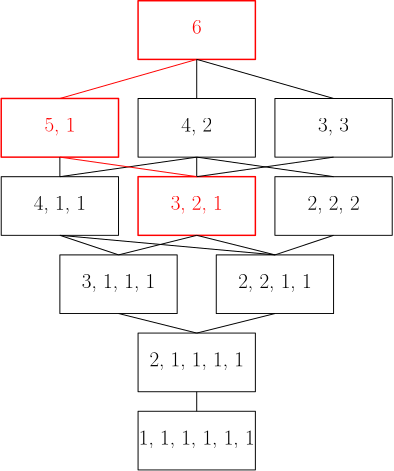
\includegraphics[width=0.8\linewidth]{images/6_firms_with_path.png}
	\caption{A chart of having 6 firms with path }
\end{figure}

\ykc{$n=6$ seems a reasonable non-trivial but not too hard example to give people ideas.}
As an example, we will use $n=6$ players under the cournot competition, as such the Nash Equilibrium of each player will be defaulted to $\frac{D}{n_C(m+1)^2}$. 

As this is a dynamic programming program, we shall start with coalition structure $\{1, 1, 1, 1, 1, 1\}$ and recursively move up each state in Figure 1. The PAR of each player is $D/49$ for some value $D$, and $V^D = D/49$ too. Therefore, $\{1, 1, 1, 1, 1, 1\}$ is a stable coalition since no player can defect by leaving their coalition. 

Moving up, the coalition structure is $\{2, 1, 1, 1, 1\}$. Again, the PAR of each player that are in their own coalition is $D/49$. As for the coalition with two players, their default value function $V^D$ is $D/72$ but splitting would give a $V^D$ of $D/49$ each. Therefore, splitting would be a better choice. 

As for $\{3, 1, 1, 1\}$ and $\{2, 2, 1, 1\}$. The PAR for all players in both structure would be $D/49$, as each player presumes the worse outcome can happen to them and expect that going to state $\{2, 1, 1, 1, 1\}$ will end up in state $\{1, 1, 1, 1, 1, 1\}$. At $S=\{3, 1, 1, 1\}$, $V^D(S, 3) = D/75$. Since $V^P(S, 3) = D/49$, the 3 players in the coalition will split into $\{2, 1\}$. Similarly, when $V^D(\{2, 2, 1, 1\}, 2) = D/50$ and $V^P(\{2, 2, 1, 1\}, 2) = D/49$, the 2 players in the coalition will split into $\{1, 1\}$. 

Moving onto $\{4, 1, 1\}$, the PAR for all players is $D/49$. Note that $V^D(\{4, 1, 1\}, 4) = D/64$, hence players in the coalition of 4 will split into $\{3, 1\}$ or $\{2, 2\}$. As for $\{3, 2, 1\}$, $V^D(\{3, 2, 1\}, 3) = D/48$, $V^D(\{3, 2, 1\}, 2) = D/32$ and $V^D(\{3, 2, 1\}, 3) = D/16$ which are all larger than $D/49$. Therefore, $\{3, 2, 1\}$ is a stable state as no agent has the incentive to further deviate, implying that $V^P(\{3, 2, 1\}, 3) = 48$, $V^P(\{3, 2, 1\}, 2) = D/32$ and $V^P(\{3, 2, 1\}, 3) = D/16$. Similarly for $\{2, 2, 2\}$, $V^D(\{2, 2, 2\}, 2) = D/32 > V^P(\{2, 2, 1, 1\}, 1) = D/49$. So, $\{2, 2, 2\}$ is also a stable state, and $V^P(\{2, 2, 2\}, 2) = D/32$. 

Looking into $\{5, 1\}$, $V^D(\{5, 1\}, 5) = D/45$. The coalition of 5 can decide to split into $\{4, 1\}$ or $\{3, 2\}$. Given that $V^P(\{3, 2, 1\}, 2) = D/32$, and $V^P(\{4, 1, 1\}, 1) = D/49$, 2 players of the coalition will choose to deviate from their original coalition to obtain a higher utility of $D/32$. Therefore, the PARs are $V^P(B(\{5, 1\}, 5, 2), 2) = D/32$, $V^P(B(\{5, 1\}, 5, 3), 3) = D/48$ and $V^P(\{5, 1\}, 1) = D/16$. 

With $\{4, 2\}$, $V^D(\{4, 2\}, 4) = D/36$ and $V^D(\{4, 2\}, 2) = D/18$. The coalition of 2 playes have no incentive to break off as $V^P(\{4, 1, 1\}, 1) = D/49 < D/18$. However, the coalition of 4 players can break off into $\{3, 1\}$ or $\{2, 2\}$. We can consider whether a player of the coalition would deviate only, with one partner, or with 2. Given that we know $V^P(\{3, 2, 1\}, 1) = D/16$, $V^P(\{2, 2, 2\}, 2) = D/32$, and $V^P(\{3, 2, 1\}, 3) = D/48$, the player shall maximise from all of the $V^Ps$, and choose to deviate by themselves, $V^P(\{3, 2, 1\}, 1)$. Therefore, the PARs are $V^P(\{4, 2\}, 2) = D/32$, $V^P(B(\{4, 2\}, 4, 3),3) = D/48$ and $V^P(B(\{4, 2\}, 4, 1), 1) = D/16$. 

Last one in this layer, $\{3, 3\}$, coalitions can only choose to break off to $\{2, 1\}$ or remain the same. Given that $V^P(\{3, 2, 1\}, 1) = D/16$ and $V^P(\{3, 2, 1\}, 2) = D/32$, players would maximise by choosing to deviate alone, $V^P(\{3, 2, 1\}, 1) = D/16$. Therefore, the PAR for each would be $V^P(\{3, 3\}, 3) = D/48$, $V^P(B(\{3, 3\}, 3, 2), 2) = D/32$, and $V^P(B(\{3, 3\}, 3, 1), 1) = D/16$. 

Finally, $\{6\}$ can choose to break off into $\{5, 1\}, \{4, 2\}$ and $\{3, 3\}$. Firstly, we find the minimum of each PAR for splitting alone, 2, 3, 4, and 5, which is as follows: 
\begin{itemize}
	\item $V^P(B(\{6\}, 6, 1), 1) = D/16$
	\item $V^P(B(\{6\}, 6, 2), 2) = D/32$ 
	\item $V^P(B(\{6\}, 6, 3), 3) = D/48$
	\item $V^P(B(\{6\}, 6, 4), 4) = D/48$
	\item $V^P(B(\{6\}, 6, 5), 5) = D/48$
\end{itemize}
Therefore, a player will choose to deviate on their own to maximise their profit. Hence, $\{6\}$ will break into $\{5, 1\}$ into $\{3, 2, 1\}$. The path is highlighted in red in Figure 1. 

\subsection{Blocking}

\ykc{Define sequential blocking. Compare with sequential blocking using the ``minimal'' example.}
Blocking is where every member of the blocking coalition is strictly better off than before leaving their previous coalition. This is done such that the blocking coalition has an improvement, while the remaining coalition is blocked from obtaining the higher utility from previously. Formally, blocking is defined as follows. Let $u$ be an allocation for a set of players $S$. We say that $(T, u')$ blocks $u$ if $T$ is a subcoalition of $S$, $(\emptyset \neq T \ S)$, $u'$ is feasible for $T$, and $u' \gg u^T$. In this case we say $u$ is blocked and that $T$ is the blocking coalition. If no such coalition exists, then $u$ is unblocked.  

\subsection{Sequential Blocking} 
An game theory terminology close to our model is sequential blocking. Let a coalition structure be $\pi$, and $a$ is the coalition equilibrium under $\pi$. The residual of any coalition in $\pi$ belongs in $\pi'$, and $a'$ is the coalition equilibrium under $\pi'$. Now, we say that $(\pi', a')$ sequentially blocks $(\pi, a)$ if there exists a sequence $\{(\pi^0, a^0), (\pi^1, a^1), \dots (\pi^m, a^m)\}$ such that 
\begin{enumerate}
	\item $(\pi^0, a^0) = (\pi, a), (\pi^m, a^m) = (\pi', a')$, and for every $i = 1, \dots, m$, there is a coalition $S^i$ that includes $(\pi^i, a^i)$ from $(\pi^{i-1}, a^{i-1})$. 
	\item $u_{S^i}(a')\gg u_{S^i}(a^{i-1})$ for all $i = 1, \dots, m$. 
\end{enumerate}
In this definition, it is only required that the utility $u$ after breaking off a coalition must be better than before, but does not require the utility to be the best out of all options unlike our model. This implies that sequential blocking may not be as easy to predict as there can be many solutions. 

However, for our model, there only exists one solution for every game up till 100 players. The model that we have created is an improvement as it is easier to predict, as it has a stronger condition. Here is an example, when $n = x$ players. 
\section{Algorithm}

\ykc{runtime, memory analysis}

%%%%%%%%%%%%%%%%%%%%%%%%%%%%%%%%%%%%%%%%%%%%%%%%%%%%%%%%%%%%%%%%%%%%%%%%

%\section{Citations and References}
%  
%The use of the \BibTeX\ to prepare your list of references is highly 
%recommended. To include the references at the end of your document, put 
%the following two commands just before the `\verb|\end{document}|' 
%command in your source file:
%%
%\begin{verbatim}
%   \bibliographystyle{ACM-Reference-Format}
%   \bibliography{sample}
%\end{verbatim}
%%
%Here we assume that `\texttt{sample.bib}' is the name of your 
%\BibTeX\ file. Use the `\verb|\cite|' command to produce citations 
%to your references. Here are a few examples for citations of journal 
%articles~\cite{GrKr96,WoJe95}, books~\cite{Knu97}, articles in 
%conference proceedings~\cite{Hag1993}, technical reports~\cite{Har78},
%Master's and PhD theses~\cite{Ani03,Cla85}, online videos~\cite{Oba08}, 
%datasets~\cite{AnMC13}, and patents~\cite{Sci09}. Both citations and 
%references are numbered by default. 
%
%Make sure you provide complete and correct bibliographic information 
%for all your references, and list authors with their full names 
%(``Donald E.\ Knuth'') rather than just initials (``D.\ E.\ Knuth''). 

%%%%%%%%%%%%%%%%%%%%%%%%%%%%%%%%%%%%%%%%%%%%%%%%%%%%%%%%%%%%%%%%%%%%%%%%

%%% The acknowledgments section is defined using the "acks" environment
%%% (rather than an unnumbered section). The use of this environment 
%%% ensures the proper identification of the section in the article 
%%% metadata as well as the consistent spelling of the heading.

\begin{acks}
If you wish to include any acknowledgments in your paper (e.g., to 
people or funding agencies), please do so using the `\texttt{acks}' 
environment. Note that the text of your acknowledgments will be omitted
if you compile your document with the `\texttt{anonymous}' option.
\end{acks}

%%%%%%%%%%%%%%%%%%%%%%%%%%%%%%%%%%%%%%%%%%%%%%%%%%%%%%%%%%%%%%%%%%%%%%%%

%%% The next two lines define, first, the bibliography style to be 
%%% applied, and, second, the bibliography file to be used.

\bibliographystyle{ACM-Reference-Format} 
\bibliography{coalition}

%%%%%%%%%%%%%%%%%%%%%%%%%%%%%%%%%%%%%%%%%%%%%%%%%%%%%%%%%%%%%%%%%%%%%%%%

\end{document}

%%%%%%%%%%%%%%%%%%%%%%%%%%%%%%%%%%%%%%%%%%%%%%%%%%%%%%%%%%%%%%%%%%%%%%%%

